\documentclass[11pt,letterpaper]{article}
\usepackage[T1]{fontenc}
\usepackage[utf8]{inputenc}
\usepackage{lmodern,microtype}
\usepackage[margin=1in,headheight=15pt]{geometry}
\usepackage{amsmath,amssymb,amsthm,mathtools}
\usepackage{booktabs,tabularx,longtable,array,enumitem}
\usepackage{xcolor,listings,tikz,needspace,fancyhdr,titlesec}
\usepackage{etoolbox}
\usetikzlibrary{arrows.meta,positioning}
\usepackage{xurl}
\usepackage[colorlinks=true,linkcolor=blue!45!black,citecolor=blue!45!black,urlcolor=blue!45!black]{hyperref}
\usepackage{bookmark}
\definecolor{ink}{HTML}{19354A}
\definecolor{accent}{HTML}{217A83}
\definecolor{pale}{HTML}{F0F5F7}
\titleformat{\section}{\Large\sffamily\bfseries\color{ink}}{\thesection}{.65em}{}
\titleformat{\subsection}{\large\sffamily\bfseries\color{ink}}{\thesubsection}{.65em}{}
\pretocmd{\section}{\Needspace{6\baselineskip}}{}{}
\BeforeBeginEnvironment{lstlisting}{\par\noindent\begin{minipage}{\linewidth}}
\AfterEndEnvironment{lstlisting}{\end{minipage}\par}
\setlength{\parskip}{.38em}
\setlength{\parindent}{0pt}
\setlength{\emergencystretch}{2em}
\setcounter{tocdepth}{1}
\setlist{nosep,leftmargin=*}
\renewcommand{\arraystretch}{1.16}
\newcolumntype{Y}{>{\raggedright\arraybackslash}X}
\newcolumntype{P}[1]{>{\raggedright\arraybackslash}p{#1}}
\newcommand{\code}[1]{\nolinkurl{#1}}
\newcommand{\R}{\mathbb R}
\newcommand{\N}{\mathbb N}
\newcommand{\Z}{\mathbb Z}
\newcommand{\Q}{\mathbb Q}
\newcommand{\source}[2]{\href{#1}{#2}}
\newcommand{\decision}[1]{\par\smallskip\noindent\textbf{Recommendation.} #1\par\smallskip}
\newcommand{\status}[1]{\textbf{Evidence status:} #1}
\newtheorem{proposition}{Proposition}
\lstset{basicstyle=\small\ttfamily,columns=fullflexible,keepspaces=true,
  breaklines=true,frame=single,rulecolor=\color{accent!35},backgroundcolor=\color{pale},
  aboveskip=.7em,belowskip=.7em,showstringspaces=false}
\pagestyle{fancy}
\fancyhf{}
\fancyhead[L]{\small\sffamily Mathematical ideas and checked evidence}
\fancyhead[R]{\small\sffamily A synthesis of nine proposals}
\fancyfoot[C]{\thepage}
\hypersetup{pdftitle={Mathematical Ideas, Checked Evidence: A Unified Evaluation of Nine Proof-Language Proposals},pdfauthor={Codex, prepared for Vladimir Reshetnikov},pdfsubject={Lean proof-language synthesis and Leant implementation review}}

\begin{document}
\begin{titlepage}
\color{ink}
{\sffamily\large LANGUAGE DESIGN / RESEARCH SYNTHESIS\par}
\vspace{1.2in}
{\sffamily\bfseries\fontsize{32}{37}\selectfont Mathematical Ideas,\\Checked Evidence\par}
\vspace{.35in}
{\sffamily\Large A unified evaluation of nine proposals\\for a more natural proof language\par}
\vspace{.5in}
{\large With a source review of automatic term synthesis\\and proof tactic suggestions in Leant\par}
\vfill
\rule{\textwidth}{1pt}
\vspace{.18in}
Prepared for Vladimir Reshetnikov\par
Codex, with independent reading and review passes\par
5 September 2026 (Pacific time)\par
\vspace{.3in}
\small
Corpus: Contour, Loom, MathStep, Mathematical Intent / MPL, Mosaic, Motive,
Outline, Reason, and Spine. This is a critical design synthesis and static
implementation review. Proposed syntax and architecture are specifications;
they are not a delivered language implementation or a measured usability result.
\end{titlepage}

\section*{The decision in brief}
\addcontentsline{toc}{section}{The decision in brief}
The nine reports converge on a coherent research direction: a Lean-hosted language
whose visible units are mathematical claims and transformations, whose omitted
details become scoped proof obligations, and whose accepted work is retained as
replayable evidence. Their agreement is much stronger than their different names
suggest. It supports building one experimental infrastructure with competing
interaction policies, rather than nine separate languages.

The central opportunity is to make the boundary between a mathematical idea and
its formal realization explicit. ``Reindex this finite sum'', ``differentiate this
identity on a neighborhood'', and ``use symmetry to reduce to this case'' can be
useful language operations when they select precise theorem-backed contracts.
Changing punctuation around tactics will not by itself remove the cost of choosing
representations, discovering lemmas, or maintaining domain libraries.

Six shared commitments are directly supported by all nine reports: a Lean host;
claim-centered proof structure; contextual obligations and method contracts;
fixed mathematical meaning before proof search; frozen evidence and replay;
and evaluation against equally equipped Lean, including abstraction costs.
Appendix~\ref{app:convergence} gives a report-by-report section crosswalk.
These are nine documents supporting six design propositions, not nine independent
experiments demonstrating their effectiveness.

The main unresolved choices concern how much reconstruction happens automatically,
how strongly the system enforces the author's stated method, when representation
and witness choices require attention, and how much evidence readers should see.
This report recommends a small typed protocol and two authoring frontends, an
ordinary Lean frontend and a mathematical-step frontend, sharing the same methods,
search services, and evidence format. That experiment can determine which gains
come from the language itself.

Leant provides substantial implemented work worth reusing: structural candidate
synthesis, exact candidate verification paths, behavioral assessment with explicit
limits, provider and fragment handling, and goal-shaped advisory tactic search.
The suggestion path also exposes concrete review targets around completion status,
replay of the displayed suggestion, and isolation of speculative work. These are
implementation-level distinctions; a common vocabulary of ``verified'' must not
erase them. Section~\ref{sec:leant} evaluates both systems separately.

The next round should deliver one end-to-end finite-reindexing example, one local
differentiation example, explicit negative neighbors, and a replayable artifact.
It should answer a few discriminating questions with code and reader observations.
More elaborate surface syntax should follow evidence from that shared experiment.

\clearpage
\tableofcontents
\clearpage

\section{Corpus, method, and strength of evidence}\label{sec:method}
\subsection{What was compared}
The input is the nine TeX reports present under \code{docs/ideas} at Brainstorm
revision \code{ddbc1d4}. We read their substantive text, their status and source
notes, and relevant companions. Three independent reading passes each covered
three reports; this synthesis compares the resulting analyses against source
passages. The associated review notes and a machine-readable source register
are included with the report. The original reports remain the primary sources
for attribution~\cite{contour,loom,mathstep,mpl,mosaic,motive,outline,reason,spine}.

\begin{tabularx}{\textwidth}{@{}lY@{}}
\toprule
Report & Distinctive emphasis used in this synthesis \\
\midrule
Contour & Mathematical moves, detailed obligation ledgers, finite reindexing, and leakage-resistant evaluation.\\
Loom & Working contexts, reconstruction recipes, local calculus, and witness/specification coupling.\\
MathStep & An assertion layer above evidence, branch-sensitive constructions, and exhaustive rebuilding of induction cases.\\
MPL & Statement seals, distinction between proof and object synthesis, preservation of general hypotheses.\\
Mosaic & Three proof views, integral and counting examples, explicit levels of method conformance.\\
Motive & Domain packages, algebraic generality, argument provenance, and failure contracts.\\
Outline & Certified higher-level plans, alternative mathematical proofs, and maintenance-oriented evaluation.\\
Reason & Reconstruction contracts, explanatory limits, and a small executable evidence model.\\
Spine & Contextual holes, structural choices, stable references, and advanced analytic patterns.\\
\bottomrule
\end{tabularx}

These emphases are not exclusive feature claims. For example, many reports discuss
views, witnesses, synthesis, and replay. Their titles and provisional language names
do not establish incompatible technical designs.

\subsection{Independent authorship is not independent validation}
The reports were commissioned in parallel, but share the task, two repositories,
much prior art, and a mathematical sample heavily concentrated in FabiusFunction.
Their common architecture could reflect a productive insight, common background,
or a shared blind spot. Authorship independence, as described by the user, does
not justify probabilistic independence or a statistical confidence estimate.

We therefore count \emph{explicit report support} only for carefully delimited
features. The count says that a proposition appears in the documents. It does not
measure implementation success, novelty, reader preference, or superiority to Lean.
Absence of discussion would not count as opposition. Differences below are labeled
as competing policies, differences in emphasis, or unresolved questions; they are
not inflated into disagreements that the texts do not express.

\subsection{Design evidence versus implementation evidence}
All nine reports identify their proposed language syntax as unimplemented. Their
paper soundness arguments explain a proof-construction discipline; they do not
verify a parser, elaborator, compiler, or editor implementation. None supplies a
comparative user study establishing reduced formalization effort.

Reason's companion is a real but narrow exception to the absence of executable
artifacts: a Python model checks simply typed terms with products, scope,
claim assembly, and origin-bound replay. Its 32 tests were rerun for this synthesis
and passed. This supports those tested model behaviors only. It is neither a Lean
kernel nor a dependent proof-language prototype~\cite[\S18]{reason}.

For the additional Leant review, the local checkout's HEAD was
\code{3a40904be8a410d832d9ab6900b3d3e7b425eccb}, but its working tree contained
modified and untracked synthesis code. The reviewed source snapshot is retained
in \code{evidence/leant-reviewed-source.zip}, with file identities in the source
register. Its Djex checkout was \code{63e7b2fa46d62c633e0b5a24a463e22b9e939df4},
different from the root commit's gitlink. Selected ProveIt observations use
\code{7c4e3f109405b9805b35d27ae96bf09c7ee5f3d5}. These differ from the older ProveIt
snapshot cited by most inputs; Reason records moving source access rather than
an immutable commit. We do not silently treat these snapshots as identical.
The source register records the actual inspected files and their correspondence
to committed content. Both repositories were treated as read-only; their builds
and test suites were not run. Source inspection, the small Python test result,
and the PDF production checks are separate evidence.

\section{What needs improving in Lean?}\label{sec:diagnosis}
\subsection{Four costs with different remedies}
The reports' most useful diagnosis is more discriminating than ``Lean is verbose''.
Their examples suggest four different sources of work.

\begin{enumerate}
\item \textbf{Mathematical work.} Choosing an invariant, strengthening an induction
  motive, finding the right normal form, or proving a regularity hypothesis is
  part of the argument. A language should help express and explore this work.
\item \textbf{Representation work.} Moving between inclusive intervals and ranges,
  natural and integer coefficients, functions and series, or bundled objects and
  their values often interrupts an otherwise clear argument. Reusable, checked
  adapters can make the intended view explicit once.
\item \textbf{Proof assembly.} Introducing binders, specializing quantified facts,
  projecting conjunctions, composing maps, and closing small arithmetic obligations
  are promising targets for bounded reconstruction and synthesis.
\item \textbf{Interaction and maintenance.} Finding a theorem name, understanding a
  failed elaboration, repairing a changed instance, and recovering the reason for
  a generated step require indexing, diagnostics, stable evidence, and good editing.
\end{enumerate}

The remedy must match the cost. A new sentence form will not replace a missing
library theorem. A powerful solver may reduce authoring keystrokes while producing
an opaque argument. A domain library can make both the new language and ordinary
Lean concise. Refactoring the mathematics itself may outperform either syntax.

\subsection{Preserve what Lean already does well}
Lean already separates extensible syntax and elaboration from a small checking
core, and tactics produce terms for that core. A language hosted there can reuse
dependent types, libraries, notation, and editor metadata~\cite{lean-elab}.
Declarative proof text is also established prior art: Isar provides structured
proof commands with explicitly stated intermediate propositions~\cite{isar}.
The proposed work should be evaluated as a new integration and interaction design,
not as the invention of structured or readable formal proof.

Several reports deliberately retain compact existing Lean examples as controls:
Contour discusses already appropriate public corollaries, and MPL examines a
short scaling proof~\cite[\S2.5]{contour}\cite[\S9]{mpl}. This matters. The goal is
not to translate every successful Lean idiom into English. Existing \code{calc},
explicit theorem applications, and well-factored lemmas may already be the best
representation of a proof.

Our ProveIt spot check gives a concrete control. The current
\code{Fabius.binomial_inversion} is already an application of a triangular-kernel
framework, and the module works for sequences in an additive commutative group.
A new frontend that assumes a field would shorten some algebra while weakening
the result. The language must preserve that generality or explicitly identify the
restriction~\cite{p-binomial}.

\subsection{Naturalness has several audiences}
Concision is not the same as naturalness. An analyst, a combinatorialist, and a
category theorist use different conventions. An author searching for a proof
needs alternatives and holes; a reader needs an argument they can follow; a
maintainer needs dependencies and stable meanings. A single presentation need
not satisfy all three at once.

The reports mainly study proofs of statements whose mathematical objects and
library infrastructure already exist. They say less about \emph{definition authoring}:
introducing a quotient, a new structure, a diagram, a hierarchy of equivalences,
or local notation. That is a serious boundary of the corpus. A better proof
surface can be valuable without yet being a better language for all mathematics.
The next evaluation should include at least one task requiring a new definition,
not merely a proof with more convenient access to existing declarations.

\section{Where the reports converge}\label{sec:convergence}
\subsection{Six shared commitments}
Appendix~\ref{app:convergence} records explicit support in all nine reports for the
following six commitments. The formulation is deliberately narrower than a claim
that they agree on every detail.

\begin{enumerate}
\item \textbf{Retain Lean as the first checking host.} Build syntax, elaboration,
  method libraries, and interaction around its existing foundations. A new kernel
  is not needed to test the proposed gains.
\item \textbf{Make assertions and mathematical steps visible.} The readable source
  should name the facts, constructions, reductions, and calculations that explain
  the proof; routine proof-state manipulation can be reconstructed.
\item \textbf{Give omissions exact contexts and contracts.} Every omitted premise
  remains an obligation. A domain method specifies how checked subproofs assemble
  into the advertised result, respecting dependent scope.
\item \textbf{Fix meaning before search.} Proof search must not silently select a
  different theorem, stronger hypothesis, algebraic structure, or data object to
  make the task easier. Material interpretation choices must remain inspectable.
\item \textbf{Discover once and retain evidence.} Rebuilding a completed proof should
  check accepted work in a specified environment, rather than depend on repeating
  the original open-ended search.
\item \textbf{Compare fairly.} Charge for methods and adapters; give the Lean
  baseline the same machinery; include failed examples and maintenance tasks.
\end{enumerate}

This is a plausible common core. It is not a complete language specification:
the syntax, granularity of a step, inference policy, evidence interchange, and
reader interface remain choices.

\subsection{Three important shared distinctions}
\textbf{Proof correctness versus statement fidelity.} A proof can be valid for an
unintended statement. The reports repeatedly distinguish checking the proof from
reviewing resolved types, quantifiers, definitions, and instances. Current Lean
validation guidance likewise distinguishes theorem validity from meaning and
provides stronger checking procedures when needed~\cite{lean-validation}.

\textbf{A proof of a proposition versus a chosen object.} A type such as
\(\N\to\N\) does not specify the successor function. Synthesis of an inverse,
normalization, branch, or witness may change later mathematics. A property, a
chosen representative, or a uniqueness theorem is needed in addition to type
inhabitation. MPL and Spine make this a particularly explicit classification,
but it recurs throughout the corpus~\cite[\S12.4]{mpl}\cite[\S9.1]{spine}.

\textbf{Search failure versus refutation.} Exhausting a budget, exhausting a
structural search fragment, and proving the negation of a mathematical statement
are different outcomes. A positive candidate can be checked against the original
goal. A negative completeness claim also needs an adequate relationship between
the searched fragment and that goal. These distinctions are directly relevant to
Leant, not merely theoretical niceties.

\subsection{The omissions are shared too}
There is little empirical evidence on error recovery, learning time, multilingual
prose, accessibility, mixed text/diagram reasoning, and library extension by ordinary
mathematicians. The repeated choice of a Lean host is practical, but leaves open
whether Lean's representation and elaboration conventions themselves cause costs
that a frontend cannot remove. There is also no convincing evidence yet for how
many domain methods can coexist before name resolution and inference become
unpredictable. Consensus should guide a prototype, not close these questions.

\section{What each proposal contributes}\label{sec:profiles}
\subsection{Contour: mathematical moves with an audit trail}
Contour develops a particularly explicit path from a named move to a ledger of
premises, a structured certificate, and a release artifact. Its finite reindexing
example exposes both a bijection and summand equality; its series example keeps
composition admissibility visible. It separates logical success, conformance to
the stated move, and explanatory value~\cite[\S\S6,7,11,12]{contour}.

Its strongest methodological contribution is the requirement to exclude the target
theorem, downstream results, and answer-bearing caches when testing reconstruction~\cite[\S15.2]{contour}.
Otherwise a solver may rediscover the theorem being benchmarked by name. The
principal implementation risk is that a richly specified ledger becomes a second
formalization burden. The useful experiment is whether reusable contracts let an
author operate mostly on mathematical objects while the ledger is generated.

\subsection{Loom: contexts and recipes that retain local hypotheses}
Loom's working contexts organize facts around a neighborhood, finite index domain,
coefficient algebra, or induction scope. Recipes reconstruct conventional moves
from these typed contexts. Its differentiation example emphasizes that the equality
must hold near the point, and its witness syntax ties a chosen term to its exact
specification~\cite[\S\S4,7,8]{loom}.

This suggests a good boundary for automation: a context can index available facts,
but cannot invent customary assumptions. The risk is an implicit domain package
that becomes as hard to inspect as a global tactic configuration. Require lexical
scope, an expansion view, and an explicit record of which recipe and contextual
facts were used. Context indexing is an optimization; the actual dependent context
remains authoritative. Its formal-series case also transports rational units into
arbitrary commutative \(\Q\)-algebras without requiring a field or an injective
algebra map~\cite[\S5]{loom}.

\subsection{MathStep: structural completeness, not just algebraic brevity}
MathStep distinguishes the layer of asserted mathematics from its elaborated
evidence and includes a notable example beyond calculus and sums: reconstructing
routine branches of an induction over derivations. Its proposed operation to
rebuild the remaining constructors must cover the selected recursor exhaustively
and must be invalidated if the datatype changes~\cite[\S\S8,10.2]{mathstep}.

That is a strong test of generality. A mathematical-step language should help with
structural arguments as well as symbolic normalization. The risk is a permissive
``and similarly for the rest'' command whose accepted cases become stale. A method
must enumerate the constructors and expose the exact motive and recursive inputs.
Test it by adding a constructor, changing an index, and omitting a recursive premise.

\subsection{MPL: preserving the statement while simplifying the proof}
\emph{Mathematical Intent, Formal Evidence}, called MPL in its text, makes a
statement seal and a semantic difference view central. Its examples explain how
overstrong differentiability assumptions, a canonical replacement for an arbitrary
solution, or an unnecessarily strong coefficient structure would alter the
mathematics~\cite[\S\S6--7,12]{mpl}.

The strongest contribution is a boundary among proof-only, data-producing, and
statement-resolving synthesis. This should shape the common protocol. A seal is a
record of one resolved meaning, not a proof that the meaning is intended. The
interface must make it feasible to review that record; merely showing a hash or
a long elaborated term transfers the burden without solving the usability problem.
MPL also sketches a concrete coefficient compiler whose shifted exponential-series
rule treats support outside the valid index range separately. This is a reusable
method candidate that preserves both arbitrary coefficient algebras and boundary
cases~\cite[\S8.4]{mpl}.

\subsection{Mosaic: explicit choices about explanatory strength}
Mosaic offers three synchronized representations: the mathematical narrative, an
obligation structure, and checked evidence. Its integral flatness bound, symmetry
argument, and square-root sum give complementary mathematical tests. Most usefully,
it explicitly distinguishes a checkpoint profile from a method-constrained
profile~\cite[\S\S4,6--9]{mosaic}.

Both profiles can be logically sound. The first checks every stated claim and
permits broad reconstruction; the second also constrains how a named operation is
implemented. This is a real experimental choice rather than a superficial syntax
preference. The stricter profile can preserve the argument's structure but may
reject an illuminating alternative. Make such alternatives source edits with a
changed explanation, not silent substitutions behind the old prose.

\subsection{Motive: reusable domain packages and honest provenance}
Motive treats conventions as domain packages containing checked moves, aliases,
normalization policies, and explanation renderers. It gives useful warnings about
transport direction, algebraic assumptions, and analytic moves whose premises
constitute substantial mathematics~\cite[\S8]{motive}.

Its discussion of explanatory provenance is especially careful: forcing a lemma
name to occur in a term does not show that the lemma mattered, and normalization
can erase syntactic scaffolding. A realistic contract records the instantiated
recipe and its obligations without claiming to establish semantic indispensability
or to reconstruct a human mental process~\cite[\S9.4]{motive}. This restraint should
be adopted throughout the unified design.
Motive's Richardson mass-one example is a useful control: idiomatic Lean already
proves the normalization in two lines. Extra surface machinery needs a demonstrated
benefit even when a domain offers many attractive new abstractions~\cite[\S2.3]{motive}.

\subsection{Outline: proof plans can improve the argument itself}
Outline builds larger certified plans, including symmetry reduction and a residual
bound that brackets a root. Its square-root example changes the proof organization
to double counting instead of merely suppressing the original successor-case
arithmetic~\cite[\S\S6,7,9]{outline}.

This is a valuable reminder that the shortest natural proof may require a better
mathematical decomposition. The corresponding evaluation hazard is attributing
that improvement to the language. Give the alternative argument and its new lemmas
to the Lean baseline too. A higher-level plan earns its place by reusing a
well-specified schema across examples, not by being a disguised theorem specialized
to the demonstration.
Its symmetry contract also transports the complete hypothesis context. A symmetric
conclusion alone does not justify exchanging variables under asymmetric assumptions.

\subsection{Reason: a small executed model with a clear boundary}
Reason brings together reconstruction contracts, theorem-backed views, explicit
outcome distinctions, and publication evidence. Its small Python companion makes
some scope and evidence-boundary claims executable~\cite[\S\S10,12,18]{reason}.
This is the corpus's clearest example of moving from architectural prose to a
testable artifact while labeling its limited reach.

That model is a useful source of protocol tests. It does not demonstrate dependent
substitution, Lean integration, mathematical methods, or the proposed reading
experience. The next step should port the tested invariants into an actual host
boundary and exercise them with a real mathematical transformation. Extending the
toy checker indefinitely would be a detour from the shared Lean-hosted experiment.

\subsection{Spine: difficult contexts and stable mathematical choices}
Spine provides contextual-hole semantics, distinguishes proof/data/structural/
presentation holes, and emphasizes references that survive insertion of nearby
text. Its examples range from finite convolutions to contraction-based uniqueness
and coefficients of formal inverse germs~\cite[\S\S4--9]{spine}.

Its insistence on certifying even unused source assertions is essential: a true
final theorem does not validate every assertion printed above it. The analytic
examples are good later stress tests, but too rich for the first implementation.
Preserve their exact obligations as roadmap requirements while starting with a
smaller finite move that can expose scope, representation, and replay end to end.
The formal-root example supplies a strong later boundary test: over a general ring,
a nonzero coefficient need not be a unit. Recursive division by it therefore needs
the stronger algebraic evidence~\cite[\S2.6]{spine}.

\section{Choices that remain open}\label{sec:choices}
\subsection{Competing policies, with proposed defaults}
\begin{longtable}{@{}P{.19\textwidth}P{.34\textwidth}P{.39\textwidth}@{}}
\toprule
Choice & Benefit and cost & Proposed first experiment \\
\midrule
\endhead
Checkpoint or method contract & Checkpoints allow flexible completion. Enforced
  methods preserve the stated plan but can constrain useful alternative proofs.
  & Support both; use method conformance for named transformations and open
  reconstruction for explicitly open claims. Compare identical tasks.\\
Implicit or explicit views & Inference removes repetitive casts. Too many possible
  views can change meaning or make resolution unpredictable.
  & One lexically scoped, explicitly selected view per nontrivial representation
  change; automatic evidence for its guards.\\
Controlled syntax or free prose & Controlled syntax has reliable scope and parsing.
  Free prose is familiar but leaves mathematical interpretation underdetermined.
  & Controlled stored source; prose can suggest an editable typed draft whose
  resolved interpretation is visible.\\
Embedded or external frontend & An embedded frontend reuses Lean elaboration.
  An external frontend may offer independent tooling but duplicates semantics.
  & Lean expressions at the boundary, with a small versioned service protocol;
  defer an independent expression elaborator.\\
Search or explicit reasons & Broad search may close more goals. Explicit reasons
  improve predictability and explainability but require discovery support.
  & Bounded local search by default; accepted broader search records a concrete
  reason and its dependencies.\\
Frozen terms or scripts & Terms avoid repeating tactic search. Scripts remain
  readable and may migrate better, but replay their elaboration and automation.
  & Retain source, resolved evidence, and environment identity. Measure script
  replay and stronger evidence replay as separate modes.\\
\bottomrule
\end{longtable}

\subsection{Default inference must not redefine the task}
Inference is not uniformly dangerous or uniformly helpful. Inferring an implicit
proof that \(i\leq n\) from interval membership normally changes no mathematical
choice. Selecting a topology, branch of a root, interpretation of subtraction,
or uniform witness may change the statement. The boundary should follow the
effect of a choice, rather than whether its syntax happens to be implicit.

Lean may interleave elaboration and proof construction. ``Fix meaning first''
should therefore mean a defined export and search boundary, not a claim that all
frontends can resolve every header in a single parser pass. An unresolved
meaning-bearing parameter can be exposed or left pending. A solver must not fill
it merely because one instantiation makes the proof easier.

\subsection{References after edits: a concrete policy difference}
Loom favors retaining resolved identities for natural references, while Outline
gives lexical rules for expressions such as ``this'' and requires review when
meaning changes~\cite[\S3]{loom}\cite[\S5]{outline}. Inserting an inequality above
``by the previous inequality'' distinguishes the policies: should the reference
stay attached to its accepted node, or follow the newly preceding statement?
Neither behavior is universally self-evident. Prefer stable stored identities
for accepted references, and display a source-level change when the author asks
for lexical retargeting. Test insertion, deletion, and copy/paste rather than
settling this question with a parser convention alone.

\subsection{Bounded automation is an interaction contract}
A budget belongs to the operation the user experiences, not only to each leaf
tactic. Twenty short probes can still create a long pause. A useful service needs
a total deadline, candidate and checking limits, cancellation, and separate
outcomes for unsupported input, exhausted budget, rejected candidate, and success.
Expensive discovery can continue asynchronously only with a stable origin and a
rule that prevents stale results from modifying a newer proof state.

\decision{Adopt a small shared semantic boundary now. Treat inference aggressiveness,
method conformance, and evidence display as testable policies above it. Do not
select a new language name or a universal default by counting report titles.}

\clearpage
\section{A common architecture and its actual guarantees}\label{sec:architecture}
\subsection{From source to evidence}
\begin{center}
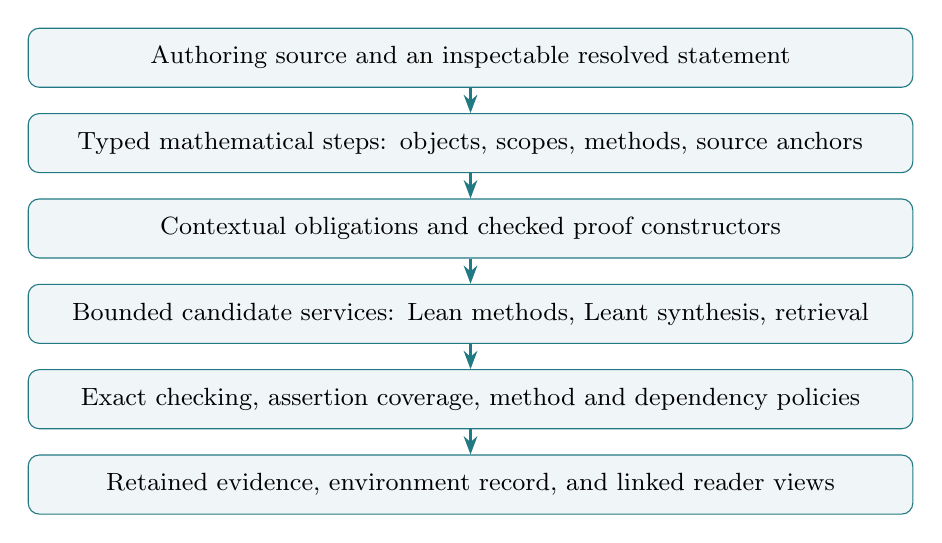
\begin{tikzpicture}[node distance=.32cm,
 box/.style={draw=accent,rounded corners,fill=pale,text width=11cm,align=center,
 minimum height=.75cm,font=\small}, >={Stealth}]
\node[box] (a) {Authoring source and an inspectable resolved statement};
\node[box,below=of a] (b) {Typed mathematical steps: objects, scopes, methods, source anchors};
\node[box,below=of b] (c) {Contextual obligations and checked proof constructors};
\node[box,below=of c] (d) {Bounded candidate services: Lean methods, Leant synthesis, retrieval};
\node[box,below=of d] (e) {Exact checking, assertion coverage, method and dependency policies};
\node[box,below=of e] (f) {Retained evidence, environment record, and linked reader views};
\foreach \x/\y in {a/b,b/c,c/d,d/e,e/f} \draw[->,thick,accent] (\x)--(\y);
\end{tikzpicture}
\end{center}
The diagram is a specification, not an implemented pipeline. Search can propose
objects for several stages, but cannot grant them authority merely by returning
success. The checking path retains the target fixed independently of the candidate.

\subsection{A minimal obligation interface}
For a fixed declaration environment \(\mathcal E\), represent an obligation as
\[
 O=(\mathit{id},\Gamma,T,\mathcal D,\mathcal P,\mathit{origin}),
\]
where \(\Gamma\) is an ordered dependent local context, \(T\) is the expected type,
\(\mathcal D\) is the allowed dependency information, \(\mathcal P\) is a search
and acceptance policy, and the origin identifies the statement, source node, and
environment. A successful candidate provides \(\mathcal E;\Gamma\vdash t:T\),
with the additional policy receipts kept distinct from that typing judgment.

The ordered context matters. In \(\forall x\,\exists y\,R(x,y)\), the witness may
depend on \(x\). In \(\exists y\,\forall x\,R(x,y)\), it may not. Closing a goal
over its telescope before sending it to an external provider makes the dependency
explicit. Restricting premises also requires retaining dependencies needed to
type the remaining context; a list of permitted printed names is insufficient.
Two visually separate goals may still share a witness, type metavariable, or
instance constraint. They can be solved independently only through closed typed
interfaces or a transactional assignment discipline that commits compatible
substitutions and restores failed alternatives. A proof-obligation DAG alone
 does not capture all elaboration constraints~\cite[\S8.3]{loom}\cite[\S9.6]{contour}.

A service response should distinguish at least:
\begin{lstlisting}
Candidate(exact_term, exact_origin)
Refinement(child_obligations, typed_combiner)
Unsupported(reason)
BudgetExhausted(budget, observations)
FragmentExhausted(fragment, completeness_evidence)
Rejected(candidate, diagnostic)
Checked(proof_receipt, policy_receipts)
\end{lstlisting}
An exact proof of a negation can be represented as checked evidence for that
negation. It is not inferred from \code{BudgetExhausted}. A fragment result keeps
its fragment and adequacy assumptions even when its internal search is complete.

\subsection{What the repeated soundness arguments amount to}
Once unresolved type and instance constraints permit such a checked interface,
represent an unfinished proof as a typed dependent function
\[
 K : \Pi(o_1:Q_1)\cdots(o_m:Q_m).\,T_\star,
\]
where each \(Q_i\) closes over its authorized local variables and may depend on
earlier obligations. The theorem type \(T_\star\) is fixed and contains no free
obligation parameters. These parameters are holes to solve, not axioms.

\begin{proposition}[Conditional assembly]
If \(K\) is well typed, and each \(p_i\) has the type \(Q_i\) after substitution
of the preceding accepted arguments, then \(Kp_1\cdots p_m:T_\star\).
\end{proposition}
\begin{proof}
Repeated dependent function application substitutes each checked argument into
the remaining telescope. The required type for the next argument is exactly the
substituted type in the hypothesis. After the final application, the remaining
type is the fixed target. Ordered, well-scoped substitution prevents use of an
unavailable variable; a dependency order prevents circular completion.
\end{proof}

This common argument is useful but modest. It is essentially the host type
theory's composition property. The hard engineering work is preserving its
hypotheses through parsing, elaboration, substitution, cache reuse, and export.
Final rechecking protects against producer mistakes; it does not prove that a
display renderer, search policy, or statement interpretation is faithful.

\subsection{Four acceptance properties, not one green light}
\begin{enumerate}
\item \textbf{Target fidelity:} the proof is checked against the intended resolved
  target in the specified environment. Equality of printed text is insufficient.
\item \textbf{Logical evidence:} the target has checked evidence under a disclosed
  transitive axiom policy, without unresolved holes or unauthorized assumptions.
\item \textbf{Document coverage:} every asserted source claim, including an unused
  intermediate claim, has evidence in its declared scope.
\item \textbf{Method conformance:} a method-constrained node was assembled using
  its declared contract, with its actual inputs and obligations recorded.
\end{enumerate}
Human explanatory quality remains a fifth, empirical judgment. A valid proof of
the final theorem could coexist with a false unused sentence in the document.
Certifying every asserted formal claim fixes that particular problem. It still cannot prove
that the argument is illuminating or that a cited lemma was indispensable.

The same separation applies to operational trust. A producer that emits terms
can be logically untrusted, but executing its metaprograms in the checking
process grants operational capabilities. A publication workflow should choose a
checking boundary appropriate to its input; it should not describe shared-process
execution as sandboxed simply because the output is later typechecked. Existing
Lean tooling already provides several levels of proof validation~\cite{lean-validation}.

\subsection{What to freeze, and what can change}
Retain the resolved target and relevant definitions, context and instance choices,
source anchors, instantiated methods, accepted terms or a defined export form,
dependency and axiom inventories, and the environment needed to replay them.
Search logs are optional diagnostics; they are not the evidence itself.

A successful tactic script is useful but may rerun simplification, typeclass
search, or theorem search. Stronger evidence replay has a different cost and
compatibility boundary. Neither mode promises byte-for-byte stability across
arbitrary Lean or library versions. Cache identity must include semantic inputs,
and a cache hit must still have an acceptance policy. Hashes identify records;
they do not establish truth or equivalence of changed declarations.

\section{Shared mathematical tests that expose the design}\label{sec:examples}
The following derivations are mathematical explanations and proposed language
tests. Their pseudocode has not been compiled as a new language. Each pairs a
useful positive case with a nearby invalid or meaning-changing case.

\subsection{Finite reindexing: make the map the visible choice}
For natural numbers \(j\leq n\), put \(m=n-j\). All sums in this example take values in \(\Z\). The map \(i\mapsto j+i\) is a bijection from
\(\{0,\ldots,m\}\) to \(\{j,\ldots,n\}\). Binomial orthogonality reduces to
\begin{align*}
 &\sum_{k=j}^{n}(-1)^{n-k}\binom nk\binom kj\\
 &\qquad=\binom nj\sum_{i=0}^{m}(-1)^{m-i}\binom mi
 =\binom nj\,[m=0]=[n=j].
\end{align*}
Here \([P]\) is one if \(P\) holds and zero otherwise. The identity
\(\binom n{j+i}\binom{j+i}j=\binom nj\binom mi\) uses \(n=j+m\).
The case \(n<j\) must be handled separately by the empty interval. It is not
covered by pretending that natural subtraction is integer subtraction.

\begin{lstlisting}
case j <= n:
  put m := n - j
  reindex the sum by i |-> j + i, from [0..m] to [j..n]
  use the binomial product identity at each i
  conclude by the alternating binomial row identity
case n < j:
  conclude because the interval is empty
\end{lstlisting}

A reindexing contract requires membership, injectivity, coverage, and equality
of corresponding summands; it retains factor order unless a commutativity theorem
permits changing it. Bounds can discharge natural-subtraction identities locally.
The current ProveIt source makes these ingredients visible through interval/range
conversion, \code{Nat.choose_mul}, arithmetic, and cast transport. Its final
transform theorem already reuses a general kernel calculus~\cite{p-binomial}.

\textbf{Negative neighbor.} Replace \([0..m]\) with \([0..m)\). The map now loses
the upper endpoint. The method must identify failed coverage, not ask a broad
solver to prove the original result by another route while retaining ``reindex''
as the explanation. Also test an infinite sum: the finite contract grants no
right to rearrange it.

\textbf{Evaluation implication.} This is an excellent first vertical slice because
it combines a meaningful explicit choice with routine guards. It is not evidence
of a language gain unless ordinary Lean receives the same reindexing API.

\subsection{Local differentiation: the neighborhood is part of the idea}
Let \(W,\varphi,G_n,G'_n:\R\to\R\). Suppose \(U\subseteq\R\) is open,
\(W\) has derivative \(\varphi(W(x))\) at every \(x\in U\), and
\(G_0(W(x))=W(x)\). Suppose, at the values \(W(x)\) actually reached for
\(x\in U\), that \(G_n\) has derivative \(G'_n\) and
\[
 G_{n+1}(W(x))=G'_n(W(x))\varphi(W(x)).
\]
Induction gives \(W^{(n)}(x)=G_n(W(x))\) on \(U\). In the successor step the
induction identity holds in a neighborhood of each \(x\in U\), so derivative
congruence and the chain rule give
\[
 W^{(n+1)}(x)=G'_n(W(x))W'(x)=G_{n+1}(W(x)).
\]
Loom, MathStep, and MPL study this autonomous-derivative pattern; Reason's affine-orbit
example requires the same neighborhood-equality distinction. The inspected
\code{AutonomousODE.iteratedDeriv_eq_comp} creates an eventual equality using
\code{hs.mem_nhds hx}, then applies derivative congruence and composition.
Its hypotheses require differentiability only at the relevant range values,
not everywhere~\cite{p-ode}.

\begin{lstlisting}
induct n, retaining the identity on U
at x in U:
  differentiate the induction identity near x
  use the chain rule and the two recurrence hypotheses
\end{lstlisting}

\textbf{Negative neighbor.} The functions \(f(t)=0\) and \(g(t)=t\) agree at
zero but have different derivatives there. A pointwise equality cannot satisfy
the neighborhood-equality premise. A diagnostic should request locality, rather
than add global differentiability or claim the theorem is false.

\textbf{Evaluation implication.} Count preserved hypothesis generality as a
correctness requirement. Compare the failure explanation for the pointwise
variant and the amount of author input needed to express the local context.

\subsection{Exact arithmetic: derive guards from a counting balance}
For \(n\in\N\), let \(s=\lfloor\sqrt n\rfloor\) and
\(S(n)=\sum_{k=1}^{n}\lfloor\sqrt k\rfloor\). Count the finite pairs
\[
 A=\{(j,k):1\leq j\leq s,\ j^2\leq k\leq n\}.
\]
For fixed \(k\), there are \(\lfloor\sqrt k\rfloor\) choices of \(j\).
For fixed \(j\), there are \(n-j^2+1\) choices of \(k\). Since \(j^2\leq n\),
all these counts are nonnegative. Thus
\[
 S(n)=\sum_{j=1}^{s}(n+1-j^2),\qquad
 S(n)+Q=s(n+1),\quad Q=\sum_{j=1}^{s}j^2.
\]
The standard square-sum identity \(6Q=s(s+1)(2s+1)\) supplies both the exact
division and, from the balance, the order needed for natural subtraction:
\[
 S(n)=s(n+1)-\frac{s(s+1)(2s+1)}6.
\]
This remains valid at \(n=0\), when both index sets are empty.

Mosaic, Outline, and Reason use this family of examples to show how a better
argument can make side conditions consequences of one central relation. The
inspected ProveIt implementation instead proves a rational formula by successor
cases, proves divisibility and a subtrahend bound, then transports back to
naturals~\cite{p-sqrt}. The counting proof is an alternative mathematical route,
not a description of that source's implementation.

\textbf{Negative neighbor.} \(\operatorname{cast}(2-3)=-1\) is false when the
subtraction inside the cast is natural subtraction: the left side is zero.
Similarly, casting natural \(1/2\) does not produce the rational number
\(1/2\). The view must retain the order and divisibility requirements, or use
a different explicitly stated operation.

\textbf{Evaluation implication.} Offer the same double-counting lemma and proof
plan to both frontends. Compare the total development cost, not a new short
proof with the old long proof while giving only the former a better theorem.

\subsection{Object selection: two roots are not interchangeable proofs}
For \(a>0\), the equation \(y^2=a\) has two real solutions. A solver asked for
\(y\) with that property may return either. If later mathematics calls the
chosen object the positive branch, the specification must also require
\(0<y\), or the author must name the branch explicitly. A type-correct inhabitant
of \(\{y:\R\mid y^2=a\}\) has not established positive-branch intent.

\begin{lstlisting}
choose r satisfying r > 0 and r*r = a
  using the positive-root construction
retain r and its specification as one accepted choice
\end{lstlisting}

MathStep's algebraic-branch case, MPL's arbitrary-versus-canonical solution
distinction, and Spine's structural holes illuminate the same issue at different
scales. Existence in \code{Prop}, construction of a dependent pair in \code{Type},
and noncomputable choice also have different elimination and policy requirements.
The word ``choose'' must not conceal which interface is being used.

\textbf{Negative neighbor.} A later optimization replaces \(r\) by \(-r\) because
both satisfy the equation. The retained positivity evidence and downstream target
no longer apply. Rechecking the new object against the full contract must fail.

\textbf{Evaluation implication.} Test visible semantic changes, not just theorem
closure. A helpful system preserves an accepted choice and explains alternatives
without allowing search success to decide the meaning of subsequent text.

\section{Review of Leant's implemented work}\label{sec:leant}
\status{Static inspection of the recorded local working-tree source, documentation,
and tests, including uncommitted changes. No Leant build, backend execution, or regression suite was
run in this review. Findings below distinguish observed code paths from proposed
runtime tests.}

\subsection{Two related systems with different jobs}
Leant's \code{:synth} constructs terms for a requested type using structural
synthesis and additional provider/assessment machinery. Its proving interface
instead starts from a live Lean proof state and proposes tactic steps shaped by
the current goal. These complement one another but are not one interchangeable
service~\cite{l-readme,l-main}.

Term synthesis is particularly relevant to reconstructing applications,
introductions, projections, and other typed assembly once the mathematical
premises are available. Tactic suggestions operate closer to the user's next
editing action: an introduction, a case split, an induction, or a closing tactic.
A future mathematical-step frontend should retain both capabilities and expose
the distinction in its protocol.

\subsection{Term synthesis: the valuable boundary is richer than ``typecheck''}
The implemented structural fragment is richer than simple implication composition:
it represents products and sums, quantified sorts, proper-type applications,
instance/provider constraints, and supported constructor families. Term-indexed
dependencies and unsupported content can remain opaque. Djinn and Exference have
different search and negative-evidence behavior; Exference is heuristic, while
Djinn's negative conclusion is qualified by projection completeness, unsafe atoms,
and budget policy. The default Djinn choice budget is not uniformly bounded, so
an adapter must impose its own complete resource policy~\cite{l-engine,l-fragment}.

The inspected implementation distinguishes rendered variants of one semantic
candidate and counts accepted candidate groups toward a quota. Its verification
scheduler is lazy: zero quota does not inspect candidate input, and successful
quota completion need not force the remaining stream. This is useful for bounded
interactive work. The \code{Verified} wrapper has a deliberately narrow contract:
it records acceptance by a supplied callback, not a solver certificate, behavioral
proof, or kernel proof~\cite{l-verification}.
The preparation and rendering pipeline retains the source/search relationship,
provider bindings, and typed candidate origin. Post-verification selection uses
scoped occurrence handles and checks permutations rather than trusting a new list
of equal-looking strings. Ranking profiles include balanced, compact, diverse,
and legacy choices; their structural costs help order candidates but do not prove
minimality or explanatory quality~\cite{l-engine,l-post,l-quality}.

Fragment translation and provider handling recognize that a structural search
engine does not understand all of Lean. Hidden structure and unsupported forms
affect what can be concluded from failure. The README qualifies complete-search
claims by the translated, provider-free structural calculus and describes
bounded provider exploration separately~\cite{l-fragment,l-readme}.

The behavioral path addresses a different question from inhabitation: whether
a candidate meets the intended specification in the assessed problem. This is
essential when several terms share a type. A constant failure function can inhabit
an option-binding type, and a state transformer can typecheck while threading the
wrong state. Behavioral assessment, rejection, inconclusive outcomes, and actual
proof evidence must retain their respective authorities rather than collapse into
a single ``good term'' flag.

\subsection{Two behavioral mechanisms, with different evidence}
The established Length model reasons about a restricted language of finite
list-spine lengths, scalar and pair domains, and linear-integer queries. Ranking
normally retains candidates; filtering needs its own authority, with independently
replayed negative evidence. Raw solver outcomes and finite positive samples do
not automatically authorize rejection or establish a universal specification of
the Lean function~\cite{l-length}.

The current uncommitted work adds a separate query using an actual Lean proposition:
\begin{lstlisting}
:synth choose : (forall A : Type, A -> A -> A)
  where choose Nat 11 29 = 29
\end{lstlisting}
This ASCII rendering illustrates the query structure. The implementation parses
the full host terms, checks the predicate under the candidate binder with
\code{autoImplicit false}, then binds each exact candidate and attempts the
supplied proposition using \code{by decide}. A successful positive proof gives
``satisfied''; a successful proof of its negation gives ``falsified''; failure
of both remains inconclusive. Only candidates passing type and predicate checks
consume the success quota~\cite{l-behavior}.

This is a useful extension beyond an external behavioral model, but its result
means exactly the proposition asked. The example checks one input; it does not
prove that the function always returns its second argument. A finite conjunction
proves that conjunction. Infinite universal specifications may be undecidable
for this method and remain inconclusive. The feature documentation explicitly
records live six-operation synthesis acceptance as pending. Source and focused
test code exist; this review supplies no new execution receipt, and the current
verdict is not yet an archived independent specification-proof bundle.

\textbf{Reuse judgment.} Preserve Leant's candidate identity, origin, capability,
budget, and outcome work. Adapt it through a narrow protocol that receives the
exact original Lean obligation. Do not make a reduced structural representation
the authority for what theorem was proved, and do not treat provider enumeration
as complete reasoning about arbitrary dependent mathematics.

\subsection{Tactic suggestions: useful structure already implemented}
In \code{Main.hs}, \code{goalCandidates} selects plausible operations from printed
goal and hypothesis shapes. Parsing is used to propose candidates; Lean's response
then determines acceptance. The candidate list includes quick finishers,
\code{exact?}, named introductions, decomposition, branching, induction, and
simplification/search. \code{apply?} is intentionally excluded, with a documented
backend failure rationale~\cite{l-main}.

\code{suggestTactic} probes a persistent proof-state identifier without pushing
accepted probes onto the user's proof stack. It retains up to three accepted, nonclosing
candidates while looking for a closer, then tries composed finishers, including
\code{simp_all} and an arithmetic continuation. Suggestions are cached by proof-state
identifier, and \code{:suggest} can reprint the result without repeating the search.
This is a concrete improvement over selecting the first tactic that merely succeeds.

The existing \code{prove-suggest} transcript exercises conjunctions, undo, existential
decomposition, list induction, and a recursive doubling example. It provides
specific intended behaviors to preserve~\cite{l-tests}. These source fixtures were
read, not rerun; they are not fresh runtime receipts.

\subsection{Three implementation boundaries to strengthen}
\textbf{Completion evidence.} In the inspected suggestion path,
\code{probeOnce} checks fatal responses, error-severity messages, and the existence
of a successor proof state. Closing classification then uses a reduction in the
number of visible goals, with a special textual check for a remaining-subgoals
comment. It does not consult a structured \code{proofStatus} field there.
\code{cmdQed} rejects visible goals but otherwise warns if the stored script
contains the text \code{sorry} and proceeds to its save path. A warning is compatible
with draft work; it is not a strict completed-proof gate~\cite{l-main}.

There are safeguards worth preserving. Standalone \code{:qed} re-elaborates the
assembled theorem source, so it can catch a malformed stored replacement before
saving. When resuming a \code{sorry}, it instead prints replacement source for the
enclosing declaration. Draft admission is intentional and does not demonstrate a
kernel soundness defect. A distinct sealed-finish operation should apply the
stronger target and axiom policy required by the proposed language.

The review concern is precise: a response with no visible goals but unresolved
proof content must not be advertised as complete on goal count alone. A smaller
goal list also denotes current-goal progress/closure, not necessarily completion
of the entire proof. Define these statuses separately and preserve backend
completion metadata. Test missing or malformed goal fields, admitted subproofs,
unresolved metavariables, and one closed goal with others remaining. These are
proposed regression cases; this review has not demonstrated their live behavior.
The separate status has concrete protocol support: locally cached REPL v1.3.18
source checks the root term, its metavariables, kernel acceptance, and admissions
after the visible goals disappear, and reports \code{proofStatus} separately.
That source is recorded with the review; it is not a claim that every Leant
invocation uses that cached binary~\cite{l-protocol}. Likewise, the existing golden
fixture intentionally calls a two-goals-to-one transition ``closes the goal''.
Preserve that useful local outcome while withholding whole-proof completion.

\textbf{The displayed artifact.} The direct probe may succeed using a question-mark
tactic, while \code{parseTryThis} extracts different text for display. The selected
text is not independently replayed before the direct path can conclude and cache
it. Chained \code{exact?} results likewise splice displayed text under conditions
about message count and line count. Those conditions improve formatting, but do
not prove that the exact displayed replacement has the same effect~\cite{l-main}.
The actual tactic-application path also stores extracted replacement text beside
the state produced by the original tactic. Its script and state histories therefore
need the same exact-replay association, even before final publication.

Replay the exact proposed edit against the same immutable origin before describing
that edit as verified. A diagnostic message is a candidate source, not an authority
for equivalence with the command that emitted it. Test a tactic that succeeds but
prints an invalid or differently scoped suggestion, and a multiline valid suggestion
whose indentation must survive formatting.

\textbf{Speculation and responsiveness.} The per-probe heartbeat bound limits some
Lean work, but \code{probeOnce} uses the session backend. Its error branch invokes
an emergency exit if that backend fails. Persistent proof-state identifiers isolate
logical state updates; they do not isolate process failure or arbitrary effects of
executed metaprograms. Per-candidate heartbeats are also not a total user-facing
deadline~\cite{l-main,l-backend}.
The current emergency path clears stale backend identifiers and preserves the
script; isolation should retain that recovery behavior rather than replace it
with an assumption that workers never fail.

Move risky or potentially expensive generated-text replay to a disposable worker
with an exact origin and an overall budget. Return accepted source and evidence to
the live session only after checking. Test timeout, cancellation, process failure,
and a late result after undo. This is a reliability requirement for proactive help,
not a claim that every existing candidate currently fails.

\subsection{What Leant does not yet supply for the proposed language}
Leant's chronological replay planner explicitly distinguishes reuse, suffix replay,
and full replay after history replacement~\cite{l-replay}. That is a good local
session abstraction. It is not by itself a theorem-publication format with target
identity, source-assertion coverage, method certificates, transitive axiom policy,
and library-version compatibility.

Ordinary candidate checking also uses a textual goal in the current environment
with \code{autoImplicit true}. This is convenient for a permissive REPL, but it
is not the approved-expression and dependent-telescope interface proposed here.
The inspected check rejects immediate errors and admissions; a separate publication
layer must enforce the transitive axiom inventory and retain exact evidence~\cite{l-fragment,l-main}.

The language experiment therefore needs an additional layer: contextual mathematical
obligations, named method contracts, evidence linked to source assertions, stable
choices of data and structures, and a defined replay boundary. Reuse existing
engines and their tested scheduling ideas rather than prematurely rewrite all
synthesis in Lean. Keep a Lean-native adapter as an architectural option if
duplicated representations prove to be the limiting cost.

\decision{First make the accepted-candidate boundary exact and testable, especially
for displayed tactic edits. Then integrate term synthesis as one provider for
typed obligations. This builds on Leant's strongest existing work and gives the
new language an honest account of what each result establishes.}

\section{Additional ideas and refinements}\label{sec:new}
These are extensions of the combined design, not claims of historical novelty.
Some build directly on ideas already present in several reports; the additional
contribution is a more specific contract or experiment.

\subsection{A semantic change budget for automatic edits}
Classify a proposed edit by its effect, then allow automation appropriate to that
effect. Replacing a proof term for the same fixed proposition is different from
changing a witness, selecting a new local structure, or strengthening a theorem.
The reports already motivate these distinctions. A useful refinement is to expose
them as an edit protocol with four outcomes:
\begin{lstlisting}
EvidenceOnly: same resolved statement and accepted objects
PlanChange: same theorem, changed mathematical decomposition
ObjectChange: a retained witness or structure changes
StatementChange: binders, hypotheses, definitions, or conclusion change
\end{lstlisting}
The first category may be automatic within policy. The others produce a visible
mathematical difference view. A stronger induction motive is typically a plan
change; it need not alter the public theorem, but it changes the local hypotheses
and should be presented as such. This avoids conflating all edits that preserve the
final type with harmless proof plumbing.

\subsection{Compare chosen objects through explicit observations}
Full equality is sometimes stronger than downstream mathematics needs. Suppose
later claims observe a witness \(w:A\) only through functions \(o_i:A\to B_i\).
Define a scoped relation
\[
 w\sim_{\mathcal O}w'\quad\Longleftrightarrow\quad
 \bigwedge_{i=1}^{r}o_i(w)=o_i(w').
\]
If every affected downstream construction is proved to respect this relation,
then replacing a representative can be justified without pretending that the
representatives are equal. This could help with quotients, choices of coordinates,
normal forms, and constructions unique only up to a relevant equivalence.

The qualification is essential. Similar-looking uses do not establish that all
dependencies respect the relation. A first implementation should require explicit
transport lemmas and a closed set of registered observations. New observations
invalidate the replacement certificate. Dependent result types may require a
dependent transport interface, not merely equality of a few scalar projections.
This is a later research direction; the safe initial policy is to retain the
accepted witness unchanged.

\subsection{Make visibility responsive to mathematical choices}
An obligation ledger can overwhelm readers as effectively as a tactic trace.
Default visibility should depend on \emph{why} an obligation exists: show branch
choices, induction motives, new regularity assumptions, and representation-changing
guards; collapse routine proofs whose propositions are already apparent from the
local context. A bound such as \(i\leq n\) may be routine inside a bounded sum,
while domination for a limit interchange is often the central argument.

This policy should be editable by author and reader, and generated from typed
nodes rather than persuasive prose. Evaluate whether readers can locate a missing
assumption quickly. Do not optimize only for the percentage of obligations hidden:
concealing the decisive premise is a failure even if the page is shorter.

\subsection{Turn negative neighbors into the method's specification}
Every contributed method should arrive with a positive instance, a nearby failure,
and an edit that changes its applicability. Finite reindexing gets an endpoint
omission; differentiation gets a pointwise-only identity; symmetry gets asymmetric
hypotheses; arithmetic transport gets failed divisibility; induction gets a new
constructor. This develops the reports' negative-test proposals into a reusable
package interface.

The expected result must include the missing proposition and the source location,
not only ``reject''. A system that refuses everything is safe in a vacuous sense
and useless. Positive neighboring cases measure whether the method is practical;
negative cases measure whether it expresses the intended mathematics.

\subsection{Build a bilingual proof document before a standalone language}
Use the same typed step structure to render both a controlled mathematical source
and an expanded Lean view. Allow an ordinary Lean proof block as an explicit leaf
and let an author gradually replace repetitive patterns with reusable methods.
The reports already support progressive adoption; the refinement is to make the
two frontends the primary controlled experiment.

The Lean view need not be a perfect textual round trip through arbitrary Lean
metaprograms. Define the subset with round-trip guarantees and preserve opaque
escape blocks verbatim with their checked boundary. Source anchors should identify
assertion nodes rather than depend on the phrase ``the previous inequality''.
A formatter may use natural references only when it can recover that stable target.

\section{How to evaluate the proposal without rewarding hidden work}\label{sec:evaluation}
\subsection{A shared baseline and two distinct studies}
Use at least three treatments: existing idiomatic Lean; refactored Lean with the
same methods, adapters, retrieval, and synthesis providers; and the proposed
mathematical-step frontend using that identical machinery. The second comparison
isolates the incremental value of the language. The first measures the total
package improvement available to the user.

Separate an \emph{authoring study} from a \emph{reading and repair study}. Authors
need to build proofs and recover from failed attempts. Readers should explain the
argument, identify dependencies, find an invalid move, and repair a small changed
hypothesis. Randomize task order and counterbalance frontend order; record prior
Lean and subject experience. Use a held-out mathematical family so demonstrations
are not the entire evaluation set.

\subsection{Measure a vector, not a single compression score}
\begin{tabularx}{\textwidth}{@{}P{.23\textwidth}Y@{}}
\toprule
Dimension & Observable outcome \\
\midrule
Author effort & Time to an accepted proof, editing actions, failed attempts,
  and explicit mathematical choices.\\
Reader understanding & Ability to state the key idea, locate a required hypothesis,
  and identify the effect of a proposed edit.\\
Maintenance & Repair time and affected nodes after a bound, definition, instance,
  theorem name, or datatype constructor changes.\\
Generality & Exact preservation of domains, quantifier dependencies, local
  hypotheses, and algebraic structure.\\
Interaction & Median and tail latency, cancellation behavior, stale result
  handling, and total checking work.\\
Evidence quality & Assertion coverage, exact displayed-edit replay, dependency
  disclosure, and defined replay success in a pinned environment.\\
Total cost & Shared infrastructure effort, per-example adapters, proof authoring,
  and subsequent maintenance.\\
\bottomrule
\end{tabularx}

Report source length and generated proof size as descriptive measurements, not
proxies for all these outcomes. A one-line invocation of a purpose-built theorem
can be shorter without explaining more or reducing total development effort.

Let \(L\) be the cost of a genuinely reusable method package, \(A_i\) the remaining
authoring cost, and \(R_i\) maintenance cost for example \(i\). Report
\[
 C(n)=L+\sum_{i=1}^{n}(A_i+R_i)
\]
alongside each component. Amortization over held-out reuse matters; dividing an
adapter cost over arbitrarily many hypothetical future proofs does not.

\subsection{An initial benchmark with discriminating mutations}
\begin{longtable}{@{}P{.22\textwidth}P{.34\textwidth}P{.36\textwidth}@{}}
\toprule
Task family & Positive task & Mutation or comparison \\
\midrule
\endhead
Finite algebra & Reindex an inclusive binomial sum. & Remove the upper endpoint;
  preserve the original additive-group generality.\\
Local analysis & Differentiate a family identity on an open set. & Replace local
  equality by equality at one point; compare diagnosis quality.\\
Counting & Derive the square-root sum using a finite relation. & Remove exact
  division evidence; compare both frontends with the same counting library.\\
Structural proof & Rebuild an induction over derivation constructors. & Add a
  constructor or alter an index; require regenerated obligations.\\
Object construction & Select a positive root with its specification. & Attempt
  substitution of the negative root after acceptance.\\
Compact control & Reuse a short scaling or transform theorem. & Measure whether
  the new frontend adds work without improving comprehension.\\
New domain & Define a small quotient-based or algebraic object. & Assess whether
  existing views and contracts support definition authoring.\\
\bottomrule
\end{longtable}

The first two tasks are implementation gates; the others broaden the study after
those work. Existing report examples are development material. Hold out variants
and at least one domain when selecting methods. Remove the target theorem and
downstream consequences from both retrieval and the allowed dependency closure;
retain a record of the permitted environment. Inspect for hidden answer leakage
through aliases, caches, examples, and imported packages.

\subsection{Ablations that can change the decision}
Disable one capability at a time: new surface syntax; contextual fact indexing;
automatic guards; broad retrieval; method conformance; frozen evidence; and
progressive disclosure. If a gain vanishes when an adapter is removed but survives
without new syntax, attribute it to the adapter. If the stricter profile improves
reader diagnosis but harms authoring time, present that tradeoff directly.

Set go/no-go criteria before measurement. Exact targets and negative-case behavior
are hard correctness requirements. Usability thresholds should be chosen after
a pilot establishes realistic variance; invented percentages now would look
precise without being informative. Publish failed tasks and repair costs as well
as successful examples.

\section{Questions for the next iteration}\label{sec:questions}
Each question below asks for an artifact or observation that would change a design
decision. The next round should distribute competing implementations of the same
contract, not request another set of unconstrained language manifestos.

\begin{enumerate}[label=\textbf{Q\arabic*.},itemsep=.65em]
\item \textbf{What is the smallest useful mathematical step?}
  Implement finite reindexing once as a theorem wrapper, once as a structured
  method with an obligation ledger. Show the author input, errors, and evidence
  produced by each. Which additional layer reduces actual work?
\item \textbf{When should a reason constrain the proof?}
  Compare checkpoint and method-constrained modes on a valid alternative proof
  and a failed advertised method. Can readers tell which argument was checked?
  Should a changed method be an explicit source edit?
\item \textbf{Which choices may reconstruction make automatically?}
  Produce an edit classification for bounds, induction motives, root branches,
  instances, and changed hypotheses. Test a stable statement before and after
  each edit. Resolve disagreement with concrete examples.
\item \textbf{What exactly does a verified suggestion guarantee?}
  For Leant, specify and test exact displayed-source replay, current-goal versus
  whole-proof completion, incomplete response handling, timeout, and undo.
  Should the public receipt encode these distinctions?
\item \textbf{How much domain infrastructure does concision require?}
  Port the same reindexing and local-calculus contracts to at least one held-out
  theorem family. Record new lemmas and engineering time, including work needed
  to make ordinary Lean equally concise.
\item \textbf{Can views remain predictable as libraries grow?}
  Add a second plausible cast, coefficient convention, or structural instance.
  Measure whether interpretation changes, ambiguity is reported, or explicit
  scope preserves the prior meaning. Define local coherence requirements.
\item \textbf{What must an author actually inspect in a statement seal?}
  Show concise renderings for changed quantifier order, a stronger domain,
  natural versus integer subtraction, and a different branch. Ask readers to
  identify the difference without reading a raw elaborated term.
\item \textbf{Which retained artifact best supports maintenance?}
  Replay a fixed proof, then rename a lemma, change a definition, and upgrade a
  dependency in an isolated experiment. Compare scripts, retained terms, and
  method-level evidence. Record repair effort and compatibility boundaries.
\item \textbf{Does the language help introduce mathematics as well as prove it?}
  Add one definition involving a quotient, equivalence, or local structure.
  Assess whether the same semantic model supports the new object naturally,
  or whether the proposed surface only benefits existing theorem applications.
\item \textbf{What should remain visible in a published argument?}
  Compare a collapsed ledger with a view that exposes choices and substantial
  analytic premises. Measure explanation and error-localization performance,
  not subjective preference alone.
\end{enumerate}

\section{A practical next-round work plan}\label{sec:roadmap}
\subsection{One shared contract, several bounded investigations}
Agree on the obligation record, exact-target boundary, source-assertion identity,
candidate outcomes, and a minimal method certificate. Assign one owner for this
shared interface. Other work can proceed in parallel on separate contracts or
frontends without creating incompatible foundational representations.

\begin{tabularx}{\textwidth}{@{}P{.18\textwidth}YP{.27\textwidth}@{}}
\toprule
Lane & Concrete deliverable & Acceptance gate \\
\midrule
Core/evidence & Lean-hosted scoped claims, one method combiner, exact checking,
  assertion coverage, and retained origin. & Reject circular/out-of-scope claims
  and mismatched targets; replay a completed example.\\
Leant adapter & Typed candidate exchange and exact displayed-tactic replay with
  bounded workers. & Distinct completion outcomes; cancellation and stale-origin
  tests; no speculative live-state mutation.\\
Finite methods & Reindexing plus guarded arithmetic transport in both frontends.
  & Positive example and endpoint/divisibility failures; same library available
  to Lean.\\
Analysis/UI & Local differentiation contract and linked source/obligation views.
  & Preserve local hypotheses; diagnose pointwise-only equality; reader can
  locate the neighborhood premise.\\
Evaluation & Counterbalanced pilot, held-out tasks, and cost register.
  & Report authoring, comprehension, failures, and maintenance separately.\\
\bottomrule
\end{tabularx}

\subsection{Milestones and stopping rules}
\textbf{Milestone A: one complete path.} Author a short finite proof, inspect its
obligations, check all assertions, export its evidence, and replay it without
rerunning discovery. Do not expand the grammar until this path works.

\textbf{Milestone B: a semantically difficult neighbor.} Add local differentiation
and a chosen data object. Demonstrate failure of the nearby invalid variants.
This tests whether the design handles mathematical meaning, not only arithmetic.

\textbf{Milestone C: comparative evidence.} Run the shared-method frontend comparison
and a repair exercise. If improvements come mainly from library work, keep that
work and reconsider how much new syntax is justified. If the language helps
readers but costs authors, offer it as a document view rather than force it as
the only input form.

Large analytic plans, automatic extraction of reusable methods from successful
proofs, broad natural-language parsing, and observation-relative witness
replacement should wait until the smaller boundary has credible evidence.
They remain research opportunities, not prerequisites for an initial useful tool.

\section{Assessment and limits}
The most defensible synthesis is a language of \emph{explicit mathematical choices
with reconstructible formal consequences}. Lean supplies a suitable initial
checking foundation. Leant supplies implemented candidate-generation and
interaction mechanisms with useful distinctions that the new design should
preserve and strengthen. The nine reports contribute complementary examples,
contracts, and evaluation safeguards.

No report, and no synthesis of their agreement, establishes that the resulting
language will be easier to learn or maintain. The central claim remains empirical:
making a mathematical move the unit of authorship should reduce representation
and assembly work without hiding meaning. A small shared implementation, honest
Lean baselines, and carefully chosen failures can test that claim.

This document delivers a comparative design judgment, a static review of selected
current implementation paths, and a next-round experimental specification. Its
mathematical explanations were reviewed as mathematics; its new pseudocode was
not compiled in Lean; the architecture and assembly argument are not a verified
compiler metatheory. The completed PDF and its layout checks establish document
production quality, not proof-language correctness.

\appendix
\section{Report-by-report convergence crosswalk}\label{app:convergence}
The entries below identify sections explicitly supporting each shared commitment.
The six columns are: \textbf{H}, Lean host; \textbf{C}, claims/checkpoints;
\textbf{O}, scoped obligations and method contracts; \textbf{F}, fixed meaning
and object/statement fidelity; \textbf{R}, retained proof and replay;
\textbf{E}, fair evaluation including shared abstraction costs. All entries are
positive source evidence, not scores. More detailed line locators appear in
the companion register and reading notes.

\begin{center}\small
\begin{tabular}{@{}lcccccc@{}}
\toprule
Report & H & C & O & F & R & E \\
\midrule
Contour & 14.1 & 4.3 & 9, 11.1 & 9.1 & 13.4 & 15.1--3\\
Loom & 3.1, 12.1 & 3.2 & 8.1--4 & 3.4, 7.4 & 10.1 & 13.1--2\\
MathStep & 18.1 & 3.3 & 9.1, 11.3 & 4.2, 14.3 & 15 & 19\\
MPL & 16.1 & 5.2 & 5, 11.3 & 12 & 14.4 & 17\\
Mosaic & 11.1 & 4--5 & 9--10 & 5.3, 10.4 & 9.5 & 13\\
Motive & 4.2, 10 & 4 & 6.1--3 & 4.2, 9.2 & 9.5 & 11.1--3\\
Outline & 5.1, 15.1 & 4.1 & 7.1, 10 & 4.2 & 12.4--5 & 14.2--3\\
Reason & 16.1 & 3.2 & 3.4, 10 & 11.1 & 13.3 & 17\\
Spine & 15 & 3 & 7 & 7.1, 9 & 12 & 16\\
\midrule
Reports supporting & 9/9 & 9/9 & 9/9 & 9/9 & 9/9 & 9/9\\
\bottomrule
\end{tabular}
\end{center}

\section{Source and artifact map}\label{app:sources}
The synthesis is \code{docs/synthesis/unified-report.tex} and its rendered
\code{unified-report.pdf}. The companion \code{source-register.json} records source
revisions, file identities, and crosswalk locators. \code{README.md} describes
rebuilding and validation. Reading and implementation-review notes are under
\code{review-notes}. Original report files are listed below relative to
\code{docs/ideas}; their PDF neighbors are linked in the bibliography.

\begin{flushleft}\small\ttfamily
\path{contour-proof-language/contour.tex}\\
\path{loom_proof_language/loom.tex}\\
\path{MathStep/MathStep.tex}\\
\path{mathematical_proof_language/article.tex}\\
\path{mosaic_proof_language/mosaic.tex}\\
\path{motive_proof_language_article/motive.tex}\\
\path{outline_proof_language/outline_proof_language.tex}\\
\path{reason_proof_language/reason.tex}\\
\path{Spine_Proof_Language/Spine_Proof_Language.tex}
\end{flushleft}

Selected local repository inspections are identified below. These are additional
observations in this synthesis and do not retroactively change the source
provenance of the original reports. All cited implementation behavior is static
source evidence unless expressly labeled otherwise.

\begin{longtable}{@{}P{.31\textwidth}P{.61\textwidth}@{}}
\toprule
Source & Inspected mechanism or declaration \\
\midrule
\endhead
ProveIt / BinomialInversion & \code{sum_Icc_neg_one_pow_choose_mul_choose},
  \code{binomial_inversion}; interval reindexing and additive-group generality.\\
ProveIt / AutonomousIteratedDeriv & \code{AutonomousODE.iteratedDeriv_eq_comp};
  neighborhood equality and range-local derivative assumptions.\\
ProveIt / FloorSqrtSum & \code{floorSqrtSumClosedForm_cast},
  \code{sum_floor_sqrt_eq_closedForm}; exact division and subtraction guards.\\
Leant / Main & \code{goalCandidates}, \code{suggestTactic}, \code{probeOnce},
  \code{parseTryThis}, \code{cmdQed}; candidate selection, response checks,
  displayed edits, and save behavior.\\
Leant / Synth.Verification & \code{Verified}, \code{verifyCandidateGroups}; callback
  receipt and lazy quota-aware verification.\\
Leant / Synth.Fragment & Structural translation, unsupported content, and
  completeness boundaries.\\
Leant / Synth.Replay & \code{planReplay}; reuse versus suffix versus full history replay.\\
Leant / Backend, tests & Session process/request handling and the
  \code{prove-suggest} behavioral transcript.\\
\bottomrule
\end{longtable}

\clearpage
\begin{thebibliography}{99}
\raggedright
\addcontentsline{toc}{section}{References}
\bibitem{contour} \emph{Contour: A Human-Scale Proof Language over Lean}.
5 September 2026. \source{../ideas/contour-proof-language/contour.pdf}{Input report PDF}.
\bibitem{loom} \emph{Loom: A Contract-Based Language for Human-Scale Formal Proofs}.
5 September 2026. \source{../ideas/loom_proof_language/loom.pdf}{Input report PDF}.
\bibitem{mathstep} \emph{MathStep: A Proof Language of Mathematical Steps}.
5 September 2026. \source{../ideas/MathStep/MathStep.pdf}{Input report PDF}.
\bibitem{mpl} \emph{Mathematical Intent, Formal Evidence} (MPL).
5 September 2026. \source{../ideas/mathematical_proof_language/article.pdf}{Input report PDF}.
\bibitem{mosaic} \emph{Mosaic: Mathematical Intent, Explicit Obligations, and
Kernel-Checked Proof}. 5 September 2026.
\source{../ideas/mosaic_proof_language/mosaic.pdf}{Input report PDF}.
\bibitem{motive} \emph{Motive: Concise Mathematical Reasoning with Kernel-Checked
Elaboration}. 5 September 2026.
\source{../ideas/motive_proof_language_article/motive.pdf}{Input report PDF}.
\bibitem{outline} \emph{Proofs at the Scale of Ideas: An Intent-Directed,
Lean-Checked Proof Language} (Outline). 5 September 2026.
\source{../ideas/outline_proof_language/outline_proof_language.pdf}{Input report PDF}.
\bibitem{reason} \emph{Reason: A Proof Language of Mathematical Intent}.
5 September 2026. \source{../ideas/reason_proof_language/reason.pdf}{Input report PDF}.
\bibitem{spine} \emph{Spine: A Proof Language for Mathematical Intent}.
5 September 2026.
\source{../ideas/Spine_Proof_Language/Spine_Proof_Language.pdf}{Input report PDF}.
\bibitem{lean-elab} Lean team. \emph{Elaboration and Compilation}, Lean Language
Reference. \url{https://lean-lang.org/doc/reference/latest/Elaboration-and-Compilation/}.
Consulted 5 September 2026 Pacific; moving documentation, not a repository toolchain pin.
\bibitem{lean-validation} Lean team. \emph{Validating a Lean Proof}, Lean Language
Reference. \url{https://lean-lang.org/doc/reference/latest/ValidatingProofs/}.
Consulted 5 September 2026 Pacific.
\bibitem{isar} Isabelle team. \emph{Programming and Proving in Isabelle/HOL},
chapter on Isar. \url{https://isabelle.in.tum.de/dist/library/Doc/Prog_Prove/Isar.html}.
Consulted 5 September 2026 Pacific.
\bibitem{p-binomial} V. Reshetnikov et al. ProveIt,
\path{Analysis/FabiusFunction/Lean/FabiusFunction/BinomialInversion.lean}.
\source{https://github.com/VladimirReshetnikov/ProveIt/blob/7c4e3f109405b9805b35d27ae96bf09c7ee5f3d5/Analysis/FabiusFunction/Lean/FabiusFunction/BinomialInversion.lean}{Pinned source}, selected lines 43--143.
\bibitem{p-ode} ProveIt,
\path{Analysis/FabiusFunction/Lean/FabiusFunction/AutonomousIteratedDeriv.lean}.
\source{https://github.com/VladimirReshetnikov/ProveIt/blob/7c4e3f109405b9805b35d27ae96bf09c7ee5f3d5/Analysis/FabiusFunction/Lean/FabiusFunction/AutonomousIteratedDeriv.lean}{Pinned source}, lines 40--65.
\bibitem{p-sqrt} ProveIt,
\path{NumberTheory/IntegerSums/Lean/IntegerSums/FloorSqrtSum.lean}.
\source{https://github.com/VladimirReshetnikov/ProveIt/blob/7c4e3f109405b9805b35d27ae96bf09c7ee5f3d5/NumberTheory/IntegerSums/Lean/IntegerSums/FloorSqrtSum.lean}{Pinned source}, selected lines 86--163.
\bibitem{l-readme} V. Reshetnikov et al. Leant, \path{README.md}.
Reviewed working-tree version in the \source{evidence/leant-reviewed-source.zip}{source snapshot}; sections on interactive proving, synthesis, behavior, and impossibility. File digest in \code{source-register.json}.
\bibitem{l-main} Leant, \path{src/Main.hs}.
Reviewed working-tree version in the \source{evidence/leant-reviewed-source.zip}{source snapshot}; selected suggestion and proof-completion paths, lines 4704--5184 and 5412--5480. This file differs from HEAD.
\bibitem{l-verification} Leant, \path{src/Leant/Synth/Verification.hs}.
Reviewed working-tree version in the \source{evidence/leant-reviewed-source.zip}{source snapshot}; callback receipts and candidate-group scheduler. This file differs from HEAD.
\bibitem{l-fragment} Leant, \path{src/Leant/Synth/Fragment.hs}.
\source{https://github.com/VladimirReshetnikov/Leant/blob/3a40904be8a410d832d9ab6900b3d3e7b425eccb/src/Leant/Synth/Fragment.hs}{Pinned source}; selected capability and structural-translation boundaries.
\bibitem{l-replay} Leant, \path{src/Leant/Synth/Replay.hs}.
\source{https://github.com/VladimirReshetnikov/Leant/blob/3a40904be8a410d832d9ab6900b3d3e7b425eccb/src/Leant/Synth/Replay.hs}{Pinned source}; \code{ReplayPlan} and \code{planReplay}.
\bibitem{l-backend} Leant, \path{src/Leant/Backend.hs}.
\source{https://github.com/VladimirReshetnikov/Leant/blob/3a40904be8a410d832d9ab6900b3d3e7b425eccb/src/Leant/Backend.hs}{Pinned source}; request and process lifecycle.
\bibitem{l-tests} Leant, \path{test/prove-suggest.txt} and its golden output.
\source{https://github.com/VladimirReshetnikov/Leant/blob/3a40904be8a410d832d9ab6900b3d3e7b425eccb/test/prove-suggest.txt}{Pinned test input}. Inspected, not rerun for this review.
\bibitem{l-engine} Leant, \path{src/Leant/Synth/Engine.hs}.
\source{https://github.com/VladimirReshetnikov/Leant/blob/3a40904be8a410d832d9ab6900b3d3e7b425eccb/src/Leant/Synth/Engine.hs}{Pinned source}; preparation, typed origins, engine limits, and qualified negative outcomes. Selected lines 259--294, 831--840, 1119--1554.
\bibitem{l-post} Leant, \path{src/Leant/Synth/PostVerification.hs}.
\source{https://github.com/VladimirReshetnikov/Leant/blob/3a40904be8a410d832d9ab6900b3d3e7b425eccb/src/Leant/Synth/PostVerification.hs}{Pinned source}; scoped occurrence handles and checked permutations.
\bibitem{l-quality} Leant, \path{docs/candidate-quality.md}.
\source{https://github.com/VladimirReshetnikov/Leant/blob/3a40904be8a410d832d9ab6900b3d3e7b425eccb/docs/candidate-quality.md}{Pinned source}; profiles, structural costs, and limits of ranking.
\bibitem{l-length} Leant, \path{docs/length-ranking.md},
\path{src/Leant/Synth/Length/Selection/Generic.hs}, and
\path{src/Leant/Synth/Length/Integration.hs}.
\source{https://github.com/VladimirReshetnikov/Leant/blob/3a40904be8a410d832d9ab6900b3d3e7b425eccb/docs/length-ranking.md}{Pinned design/implementation documentation}; selected sources also retained in the snapshot.
\bibitem{l-behavior} Leant working tree,
\path{src/Leant/Synth/Behavioral.hs}, \path{docs/behavioral-synthesis.md},
and \path{test-unit/Spec.hs}. Uncommitted sources in the
\source{evidence/leant-reviewed-source.zip}{review snapshot}; parsing, exact proposition checks, verdicts, and stated integration-validation boundary.
\bibitem{l-protocol} Lean community REPL, locally cached source tagged
\code{repl_v1.3.18_lean-toolchain-v4.32.0}, \path{REPL/Main.lean}, lines 249--323,
and \path{REPL/JSON.lean}, lines 240--256. The
\source{evidence/repl-protocol-source.zip}{protocol source snapshot} retains these files and its license; provenance is recorded in the source register.
\end{thebibliography}
\end{document}
